\documentclass[answers]{exam}

\usepackage{amsmath, amsfonts, amssymb}
\usepackage{geometry}
\usepackage{graphics}
\usepackage{graphicx}
\usepackage{tikz}
\usepackage{listings}
\usepackage{subfig}
\usepackage{float}

\lstset{
    basicstyle=\ttfamily,
    columns=fullflexible,
    frame=single,
    breaklines=true,
    postbreak=\mbox{\textcolor{red}{$\hookrightarrow$}\space},
}

\geometry{
    bottom=2cm, % Adjust this value as needed to leave space for the answer boxes
}

% Define colors for listings
\definecolor{codegreen}{rgb}{0,0.6,0}
\definecolor{codegray}{rgb}{0.5,0.5,0.5}
\definecolor{codepurple}{rgb}{0.58,0,0.82}
\definecolor{backcolour}{rgb}{0.95,0.95,0.92}

% Setup the listings package
\lstdefinestyle{mystyle}{
    backgroundcolor=\color{backcolour},   
    commentstyle=\color{codegreen},
    keywordstyle=\color{magenta},
    numberstyle=\tiny\color{codegray},
    stringstyle=\color{codepurple},
    basicstyle=\ttfamily\footnotesize,
    breakatwhitespace=false,         
    breaklines=true,                 
    captionpos=b,                    
    keepspaces=true,                 
    numbers=left,                    
    numbersep=5pt,                  
    showspaces=false,                
    showstringspaces=false,
    showtabs=false,                  
    tabsize=2
}

\lstset{style=mystyle}

% Header and footer.
\pagestyle{headandfoot}
\runningheadrule
\runningfootrule
\runningheader{EE/CE 468/468 Mobile Robotics}{Homework 3}{Fall 2023}
\runningfooter{}{Page \thepage\ of \numpages}{}
\firstpageheader{}{}{}

\boxedpoints
\printanswers

\newcommand{\uvec}[1]{\boldsymbol{\hat{\textbf{#1}}}}
\newcommand\union\cup
\newcommand\inter\cap
\newcommand\ul\underline
\newcommand\ol\overline

\title{Assignment 3\\ EE/CE 468/468 Mobile Robotics\\ Habib University -- Fall 2023}
\author{Ali Asghar Yousuf \\ Muhammad Azeem Haider }
\date{\today}

\begin{document}
\maketitle

\begin{questions}
    \question[20]
    Consider a robot that lives in a 1-D coordinate system. Its location will be denoted by \(x\), its velocity by \(\dot{x}\), and its acceleration by \(\ddot{x}\). Suppose we can only control the acceleration \(\ddot{x}\). Making use of equations of motion from school physics, write the discrete-time motion model for this system. Assume that the acceleration \(\ddot{x}\) is a sum of a commanded acceleration and a zero-mean noise term with variance \(\sigma^2\) and assume that the actual acceleration remains constant in an interval \(\Delta t\).
    \begin{parts}
        \part Find the uncertainty/covariance in the pose \((x, \dot{x})\) after one time step. Are the two correlated?
        \begin{solution}
            Starting with the classic kinematic equations:
            \begin{align*}
                x & = v_i t + \frac{1}{2} a t^2, \\
                v & = v_i + a t,
            \end{align*}
            and transitioning to a discrete-time domain for the \( k \)-th time step, we get:
            \begin{align*}
                x_{k+1}       & = x_k + \dot{x}_k \Delta t + \frac{1}{2} \ddot{x}_k \Delta t^2, \\
                \dot{x}_{k+1} & = \dot{x}_k + \ddot{x}_k \Delta t.
            \end{align*}

            The state transition incorporating noise becomes:
            \begin{align*}
                x_{k+1}       & = x_k + \dot{x}_k \Delta t + \frac{1}{2} (a_k + \eta_k) \Delta t^2, \\
                \dot{x}_{k+1} & = \dot{x}_k + (a_k + \eta_k) \Delta t.
                `\end{align*}

            The acceleration includes a deterministic part and a random noise component:
            \begin{align*}
                \ddot{x}_k & = a_k + \eta_k,      \\
                \eta_k     & \sim N(0, \sigma^2).
            \end{align*}

            \[
                \Sigma = \begin{bmatrix}
                    \sigma_{xx}       & \sigma_{x\dot{x}}       \\
                    \sigma_{x\dot{x}} & \sigma_{\dot{x}\dot{x}}
                \end{bmatrix}
            \]
            where:
            \begin{itemize}
                \item \( \sigma_{xx} \) is the variance of the position \( x \),
                \item \( \sigma_{\dot{x}\dot{x}} \) is the variance of the velocity \( \dot{x} \),
                \item \( \sigma_{x\dot{x}} \) is the covariance between position \( x \) and velocity \( \dot{x} \).
            \end{itemize}

            Assume that there are two Jacobean's $J_1$ and $J_2$ which we will find as

            \begin{equation}
                \Delta_{x} f \quad
            \end{equation}
            \begin{equation}
                \quad \Delta_{u} f
            \end{equation}
            As a result we can express our two Jacobean's in the following manner;
            \begin{align*}
                J_1 = \begin{bmatrix}
                          1 & \Delta t \\
                          0 & 1
                      \end{bmatrix} \\
                J_2 = \begin{bmatrix}
                          \dfrac{1}{2} \Delta t^2 \\
                          \Delta t
                      \end{bmatrix}
            \end{align*}
            Using the update rule we get the following equation
            \begin{equation}
                P_{k+1} = J_1 P_k J_1^T + J_2 \sum_{uu} J_2^T
            \end{equation}

            Substituting the values for Jacobean $J_1$ and $J_2$ in the equation, we get;
            \begin{align*}
                P_{k+1} = \begin{bmatrix} 1 & \Delta t \\ 0 & 1 \end{bmatrix}
                P_k
                \begin{bmatrix} 1 & 0 \\ \Delta t & 1 \end{bmatrix} +
                \begin{bmatrix} \dfrac{1}{4}\Delta t^4 \sigma^2 & \dfrac{1}{2}\Delta t^3 \sigma^2 \\ \dfrac{1}{2}\Delta t^3 \sigma^2 & \Delta t^3 \sigma^2 \end{bmatrix}
            \end{align*}
            For the purpose of our solution, we assume that the covariance at time step $P_0$ is equal to zero. This makes this part of the equation zero;
            \begin{align*}
                \begin{bmatrix} 1 & \Delta t \\ 0 & 1 \end{bmatrix}
                P_k \begin{bmatrix} 1 & 0 \\ \Delta t & 1 \end{bmatrix} & = 0
            \end{align*}

            As a result the covariance when time step is equal to one is as followed;

            \begin{align*}
                \begin{bmatrix} \dfrac{1}{4}\Delta t^4 \sigma^2 & \dfrac{1}{2}\Delta t^3 \sigma^2 \\ \dfrac{1}{2}\Delta t^3 \sigma^2 & \Delta t^3 \sigma^2 \end{bmatrix}
            \end{align*}
        \end{solution}

        \part Suppose we control this robot with a commanded acceleration sequence \(a_1, a_2, a_3, \ldots\) for \(T\) time intervals. Will the final location \(x\) and the final velocity \(\dot{x}\) be correlated for some large value of \(T\)?
        \begin{solution}
            Given the state transition matrix \( J_1 \) and the noise covariance matrix \( Q \) from part a, we can analyze the correlation between the final position \( x \) and velocity \( \dot{x} \) after \( T \) time intervals. The state covariance matrix \( P_T \) evolves according to the recursive relationship:

            \[
                P_T = J_1 P_{T-1} J_1^T + Q
            \]

            Assuming the initial covariance \( P_0 = \mathbf{0} \), the recursive expansion
            of \( P_T \) is:

            \[
                P_T = J_1^T P_0 (J_1^T)^T + \sum_{i=0}^{T-1} J_1^i Q (J_1^T)^i
            \]

            Given that \( P_0 = \mathbf{0} \), the evolution of \( P_T \) is solely due to
            the noise matrix \( Q \) being propagated through the system dynamics:

            \[
                P_T = \sum_{i=0}^{T-1} J_1^i Q (J_1^T)^i
            \]

            The off-diagonal terms of \( P_T \), \( \sigma_{x\dot{x}} \), represent the
            covariance between position \( x \) and velocity \( \dot{x} \). If \( J_1 \)
            has values with magnitude greater than or equal to one, or if \( Q \)
            introduces sufficient noise at each step, these off-diagonal terms may not
            converge to zero even as \( T \) becomes large. This implies that the final
            position \( x \) and velocity \( \dot{x} \) will be correlated, reflecting the
            cumulative effect of the process noise on the system's state over time.
        \end{solution}
    \end{parts}

    \question[20]
    Suppose we have a mobile robot operating in a planar environment. Its state is its \(x\)-\(y\) location and its global heading direction \(\theta\). Suppose we know \(x\) and \(y\) with high certainty but the orientation \(\theta\) is unknown. This is reflected in our initial estimate:
    \[
        \hat{x}_0 = \begin{bmatrix} 0 \\ 0 \\ 0 \end{bmatrix}, \quad
        \Sigma_0 = \begin{bmatrix} 0.01 & 0 & 0 \\ 0 & 0.01 & 0 \\ 0 & 0 & 10000 \end{bmatrix}.
    \]
    \begin{parts}
        \part Assume that the robot moves flawlessly without any noise. We'll consider the simple case when the robot's heading is not being controlled i.e. \(\omega = 0\). Observations of the robot are made at discrete points in time and consist of the robot's distance from the origin \(d\) and the bearing \(\theta\) measured from the origin. Assume that the noise associated with these two measurements are independent. Develop a Kalman Filter that maintains an estimate of the robot’s state.
        \begin{solution}
            % develop a kalman filter instead of an extended kalman filter
            Since the robot's heading is not being controlled and the robot moves
            flawlessly without any noise, the state transition model is given by:
            \begin{align*}
                x_{k+1}      & = x_k + v_k \Delta t \cos(\theta_k),   \\
                y_{k+1}      & = y_k + v_k \Delta t \sin(\theta_k),   \\
                \theta_{k+1} & = \theta_k.                            \\
                A_k          & = \begin{bmatrix}
                                     1 & 0 & -v_k \Delta t \sin(\theta_k) \\
                                     0 & 1 & v_k \Delta t \cos(\theta_k)  \\
                                     0 & 0 & 1
                                 \end{bmatrix} \\
            \end{align*}

            The observation model is given by:
            \begin{align*}
                d_k      & = \sqrt{x_k^2 + y_k^2} + \eta_k,                                              \\
                \theta_k & = \tan^{-1}\left(\frac{y_k}{x_k}\right) + \eta_k.                             \\
                C_k      & = \begin{bmatrix}
                                 \frac{x_k}{\sqrt{x_k^2 + y_k^2}} & \frac{y_k}{\sqrt{x_k^2 + y_k^2}} & 0
                             \end{bmatrix} \\
            \end{align*}

            The state transition noise covariance matrix is given by:
            \begin{align*}
                R_k & = \begin{bmatrix}
                            0 & 0 & 0 \\
                            0 & 0 & 0 \\
                            0 & 0 & 0
                        \end{bmatrix} \\
            \end{align*}

            The observation noise covariance matrix is given by:
            \begin{align*}
                Q_k & = \begin{bmatrix}
                            \sigma^2_{d} & 0                 \\
                            0            & \sigma^2_{\theta}
                        \end{bmatrix}
            \end{align*}

            The Kalman Filter equations are given by:

            \textbf{Prediction Step:}
            \begin{align*}
                \bar{x}_{k}      & = A_{k} \hat{x}_{k-1},       \\
                \bar{\Sigma}_{k} & = A_{k} \Sigma_{k-1} A_{k}^T
            \end{align*}

            \textbf{Update Step:}
            \begin{align*}
                K_{k}       & = \bar{\Sigma}_{k} C_{k}^T \left(C_{k} \Sigma_{k} C_{k}^T + Q_{k}\right)^{-1}, \\
                \hat{x}_{k} & = \bar{x}_{k} + K_{k} \left(z_{k} - C_{k} \bar{x}_{k}\right),                  \\
                \Sigma_{k}  & = \left(I - K_{k} C_{k}\right) \bar{\Sigma}_{k}.
            \end{align*}
        \end{solution}

        \part The location of the robot is a random vector. Draw 1000 samples of the initial state from a Gaussian distribution of the stated mean and covariance, propagate each initial state sample according to the motion equation and plot the samples of the \(x\)-\(y\) state only at time 1 in MATLAB. Assume that distance covered in one time step is 1.
        \begin{solution}
            The following figure shows the 1000 samples of the initial state propagated
            according to the motion equation at time 1.
            \begin{figure}[H]
                \centering
                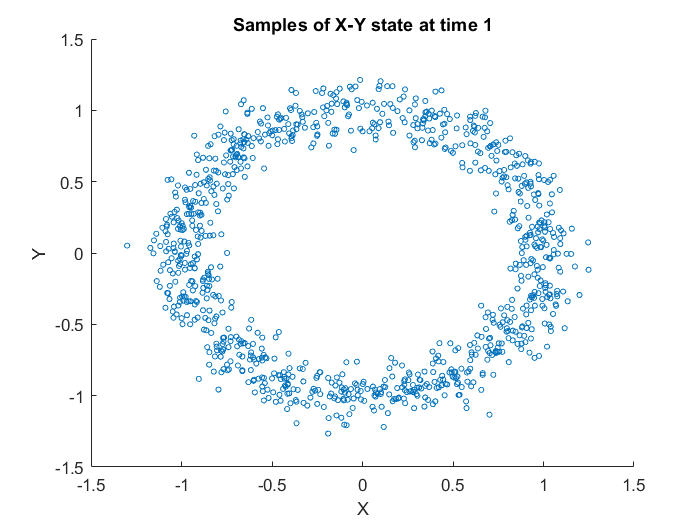
\includegraphics[width=0.8\textwidth]{images/2b.png}
                \caption{1000 samples of the initial state propagated according to the motion equation at time 1.}
            \end{figure}
        \end{solution}

        \part Use the prediction step of the EKF to make a prediction about the state at time 1 and its corresponding covariance. Plot the uncertainty ellipse of a Gaussian with mean equal to \(\bar{x}_1\) and covariance \(\bar{\Sigma}_1\) on the same plot as (a) and compare and comment on the two.
        \begin{solution}
            Using the prediction step of the EKF:
            \begin{align*}
                \bar{x}_{k}      & = g(\hat{x}_{k-1}),                            \\
                \bar{\Sigma}_{k} & = G_{k} \Sigma_{k-1} G_{k}^T
                \intertext{where}
                G_{k}            & = \begin{bmatrix}
                                         1 & 0 & -v_{k-1} \Delta t \sin(\theta_{k-1}) \\
                                         0 & 1 & v_{k-1} \Delta t \cos(\theta_{k-1})  \\
                                         0 & 0 & 1
                                     \end{bmatrix} \\
                \Delta t         & = 1                                            \\
                v_0              & = 1                                            \\
                \theta_0         & = 0                                            \\
                \hat{x}_{0}      & = \begin{bmatrix}
                                         0 \\ 0 \\ 0
                                     \end{bmatrix}                               \\
                \Sigma_{0}       & = \begin{bmatrix}
                                         0.01 & 0    & 0     \\
                                         0    & 0.01 & 0     \\
                                         0    & 0    & 10000
                                     \end{bmatrix}                          \\
            \end{align*}

            Putting the values in the above equations, we get:
            \begin{align*}
                \bar{x}_{1}      & = \begin{bmatrix}
                                         \hat{x}_{0} + v_0 \Delta t \cos(\theta_0) \\
                                         \hat{y}_{0} + v_0 \Delta t \sin(\theta_0) \\
                                         \hat{\theta}_{0}
                                     \end{bmatrix}
                = \begin{bmatrix}
                      0 + (1)(1)\cos(0) \\ 0 + (1)(1)\sin(0) \\ 0
                  \end{bmatrix}
                = \begin{bmatrix}
                      1 \\ 0 \\ 0
                  \end{bmatrix},                                                                                                \\
                \bar{\Sigma}_{1} & = \begin{bmatrix}
                                         1 & 0 & -v_0 \Delta t \sin(\theta_0) \\
                                         0 & 1 & v_0 \Delta t \cos(\theta_0)  \\
                                         0 & 0 & 1
                                     \end{bmatrix} \begin{bmatrix}
                                                       0.01 & 0    & 0     \\
                                                       0    & 0.01 & 0     \\
                                                       0    & 0    & 10000
                                                   \end{bmatrix} \begin{bmatrix}
                                                                     1                            & 0                           & 0 \\
                                                                     0                            & 1                           & 0 \\
                                                                     -v_0 \Delta t \sin(\theta_0) & v_0 \Delta t \cos(\theta_0) & 1
                                                                 \end{bmatrix} \\
                                 & = \begin{bmatrix}
                                         1 & 0 & 0 \\
                                         0 & 1 & 1 \\
                                         0 & 0 & 1
                                     \end{bmatrix} \begin{bmatrix}
                                                       0.01 & 0    & 0     \\
                                                       0    & 0.01 & 0     \\
                                                       0    & 0    & 10000
                                                   \end{bmatrix} \begin{bmatrix}
                                                                     1 & 0 & 0 \\
                                                                     0 & 1 & 0 \\
                                                                     0 & 1 & 1
                                                                 \end{bmatrix}                                                 \\
                                 & = \begin{bmatrix}
                                         0.01 & 0     & 0     \\
                                         0    & 10000 & 10000 \\
                                         0    & 10000 & 10000
                                     \end{bmatrix}
            \end{align*}

            The uncertainty ellipse of a Gaussian with mean equal to \(\bar{x}_1\) and
            covariance \(\bar{\Sigma}_1\) is shown in the following figure:
            \begin{figure}[H]
                \centering
                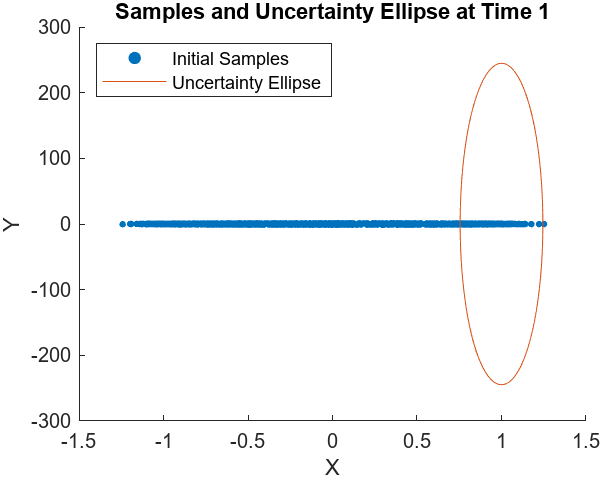
\includegraphics[width=0.8\textwidth]{images/2c.png}
                \caption{Uncertainty ellipse of a Gaussian with mean equal to \(\bar{x}_1\) and covariance \(\bar{\Sigma}_1\).}
            \end{figure}
        \end{solution}

        \part Now incorporate a noisy measurement i.e. \(z = d + \epsilon\) where \(\epsilon\) is zero-mean with covariance 0.01. Again draw the uncertainty ellipse on the same plot after incorporating the measurement.
        \begin{solution}
            The observation model in this problem is given by:
            \begin{align*}
                z_k    & = \sqrt{x_k^2 + y_k^2} + \eta_k                                                 \\
                \eta_k & \sim N(0, \sigma^2)                                                             \\
                \intertext{We know that,}
                z_k    & = h(x_k) + \eta_k                                                               \\
                K_k    & = \bar{\Sigma}_k H_k^T \left(H_k \bar{\Sigma}_k H_k^T + Q_k\right)^{-1}         \\
                \intertext{where}
                H_k    & = \begin{bmatrix}
                               \dfrac{x_k}{\sqrt{x_k^2 + y_k^2}} & \dfrac{y_k}{\sqrt{x_k^2 + y_k^2}} & 0
                           \end{bmatrix} \\
                \intertext{Therefore, we can calculate \(K_k\) as follows:}
                K_1    & = \Sigma_1 H_1^T \left(H_1 \Sigma_1 H_1^T + Q_1\right)^{-1}                     \\
                H_1    & = \begin{bmatrix}
                               \dfrac{1}{\sqrt{1^2 + 0^2}} & \dfrac{0}{\sqrt{1^2 + 0^2}} & 0
                           \end{bmatrix}
                = \begin{bmatrix}
                      1 & 0 & 0
                  \end{bmatrix}
            \end{align*}                                                                                                 \\

            From previous calculation we know that,

            \begin{align*}
                \Sigma_1 & = \begin{bmatrix}
                                 0.01 & 0     & 0     \\
                                 0    & 10000 & 10000 \\
                                 0    & 10000 & 10000
                             \end{bmatrix}                                                                                    \\
                K_1      & = \begin{bmatrix}
                                 0.01 & 0    & 0     \\
                                 0    & 0.01 & 0     \\
                                 0    & 0    & 10000
                             \end{bmatrix} \begin{bmatrix}
                                               1 \\ 0 \\ 0
                                           \end{bmatrix} \left(\begin{bmatrix}
                                                                   1 & 0 & 0
                                                               \end{bmatrix} \begin{bmatrix}
                                                                                 0.01 & 0    & 0     \\
                                                                                 0    & 0.01 & 0     \\
                                                                                 0    & 0    & 10000
                                                                             \end{bmatrix} \begin{bmatrix}
                                                                                               1 \\ 0 \\ 0
                                                                                           \end{bmatrix} + \begin{bmatrix}
                                                                                                               0.01
                                                                                                           \end{bmatrix}\right)^{-1} \\
                         & = \begin{bmatrix}
                                 0.5 \\ 0 \\ 0
                             \end{bmatrix}
            \end{align*}
            For $\hat{x}_1$,
            \begin{align*}
                \hat{x}_1 & = \bar{x}_1 + K_1 \left(z_1 - h(\bar{x}_1)\right)                   \\
                          & = \begin{bmatrix}
                                  1 \\ 0 \\ 0
                              \end{bmatrix} + \begin{bmatrix}
                                                  0.5 \\ 0 \\ 0
                                              \end{bmatrix} \left(z_1 - \sqrt{1^2 + 0^2}\right) \\
            \end{align*}

            $z_1 \sim N(1, 0.01)$, if we put in the mean we get,

            \begin{align*}
                \hat{x}_1 & = \begin{bmatrix}
                                  1 \\ 0 \\ 0
                              \end{bmatrix} + \begin{bmatrix}
                                                  0.5 \\ 0 \\ 0
                                              \end{bmatrix} \left(1 - 1\right)
                = \begin{bmatrix}
                      1 \\ 0 \\ 0
                  \end{bmatrix}
            \end{align*}
            For $\Sigma_1$,
            \begin{align*}
                \Sigma_1 & = \left(I - K_1 H_1\right) \bar{\Sigma}_1                           \\
                         & = \left(I - \begin{bmatrix}
                                               0.5 \\ 0 \\ 0
                                           \end{bmatrix} \begin{bmatrix}
                                                             1 & 0 & 0
                                                         \end{bmatrix}\right) \begin{bmatrix}
                                                                              0.01 & 0     & 0     \\
                                                                              0    & 10000 & 10000 \\
                                                                              0    & 10000 & 10000
                                                                          \end{bmatrix} \\
                         & = \begin{bmatrix}
                                 0.005 & 0     & 0     \\
                                 0     & 10000 & 10000 \\
                                 0     & 10000 & 10000
                             \end{bmatrix}
            \end{align*}

            The uncertainty ellipse of a Gaussian with mean equal to \(\hat{x}_1\) and
            covariance \(\Sigma_1\) with the measurement is shown in the following figure:
            \begin{figure}[H]
                \centering
                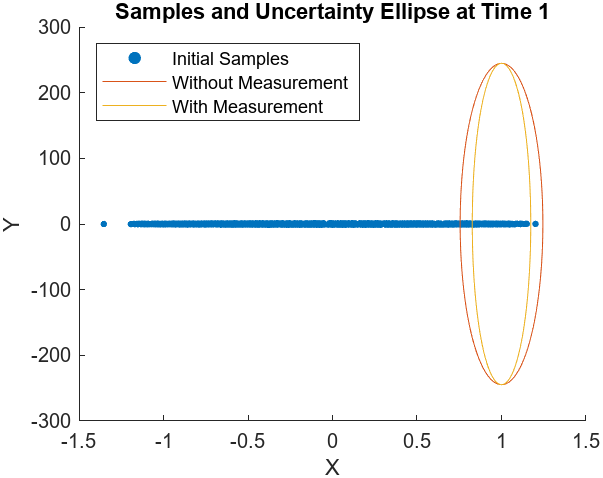
\includegraphics[width=0.8\textwidth]{images/2d.png}
                \caption{Uncertainty ellipse of a Gaussian with mean equal to \(\hat{x}_1\) and covariance \(\Sigma_1\) with the measurement.}
            \end{figure}
        \end{solution}

        \part What would have been your estimate for the \(x\)-\(y\) at time 1 considering (a)? What would be your comments about the estimate provided by the EKF? What would have happened if the initial orientation were known but we were uncertain about the \(y\) coordinate?
        \begin{solution}
            Given the scenario in part (a), where the robot moves flawlessly without any noise and the initial orientation is known, the estimate for the x-y coordinates at time 1 would solely rely on the robot's flawless motion.

            For instance, if the robot starts at the origin \((0, 0)\) with a known initial
            orientation, and it moves flawlessly in a straight line without any noise, the
            x-coordinate would change based on the distance traveled along the x-axis, and
            the y-coordinate would remain at \(0\) due to the straight-line movement.

            The EKF's estimate at time 1 is influenced by both the prediction step (motion
            model) and the measurement update (incorporating noisy measurements). In the
            provided scenario, the EKF's prediction step essentially assumes a flawless
            movement without any noise. Incorporating a noisy measurement, as done in the
            EKF, helps refine the estimate by considering sensor readings, thus potentially
            improving the accuracy of the estimate.

            If the initial orientation were known but there was uncertainty about the
            y-coordinate, the EKF would take this uncertainty into account during its
            prediction and update steps. In such a scenario, the EKF would provide an
            estimate that combines the information from the motion model and the sensor
            readings to estimate the state, considering the uncertainty about the
            y-coordinate. This would likely result in an estimate that combines the prior
            knowledge (known initial orientation) with the sensor measurements to refine
            the estimation process, leading to a more accurate estimation of the robot's
            state.
        \end{solution}
    \end{parts}

    \question[20]
    Suppose we live at a place where days are either sunny, cloudy, or rainy. The weather tomorrow is determined solely by the weather today (it’s a Markov Chain) and is captured by the following state transition probabilities:
    \begin{center}
        \textbf{Today's Weather} \\
        \begin{tabular}{|c|c|c|c|}
            \hline
            \textbf{}       & \textbf{Sunny} & \textbf{Cloudy} & \textbf{Rainy} \\ \hline
            \textbf{Sunny}  & 0.8            & 0.2             & 0              \\ \hline
            \textbf{Cloudy} & 0.4            & 0.4             & 0.2            \\ \hline
            \textbf{Rainy}  & 0.2            & 0.6             & 0.2            \\ \hline
        \end{tabular}
    \end{center}
    Suppose that we cannot observe the weather directly but instead rely on a sensor. Our sensor is noisy. The measurements are governed by the following measurement model:
    \begin{center}
        \textbf{Actual Weather} \\
        \begin{tabular}{|c|c|c|c|}
            \hline
            \textbf{}       & \textbf{Sunny} & \textbf{Cloudy} & \textbf{Rainy} \\ \hline
            \textbf{Sunny}  & 0.6            & 0.4             & 0              \\ \hline
            \textbf{Cloudy} & 0.3            & 0.7             & 0              \\ \hline
            \textbf{Rainy}  & 0              & 0               & 1              \\ \hline
        \end{tabular}
    \end{center}
    \begin{parts}
        \part Suppose Day 1 is sunny (this is known for a fact). At days 2 through 4 the sensor measures sunny, sunny, rainy. For each of the days 2 through 4 what is the most likely weather on that day. Answer the question in two ways: one in which only the data available to the day in question is used and one in hindsight where data from future days is also available.

        \begin{solution}
            \textbf{Day 2 $\mid$ only data available to the day in question is used}
            \begin{align*}
                P(x_2 \mid x_1, z_2) & = \eta P(z_2 \mid x_2, x_1) P(x_2 \mid x_1)          \\
                                     & = \eta P(z_2 \mid x_2) P(x_2 \mid x_1)               \\
                                     & = \eta \begin{bmatrix}
                                                  0.6 \\
                                                  0.3 \\
                                                  0
                                              \end{bmatrix} \cdot \begin{bmatrix}
                                                                      0.8 \\
                                                                      0.2 \\
                                                                      0
                                                                  \end{bmatrix}            \\
                                     & = \eta \begin{bmatrix}
                                                  0.48 \\
                                                  0.06 \\
                                                  0
                                              \end{bmatrix}                                \\
                                     & = \eta \left( 0.48 + 0.06 + 0 \right) \begin{bmatrix}
                                                                                 0.48 \\
                                                                                 0.06 \\
                                                                                 0
                                                                             \end{bmatrix} \\
                                     & = \frac{1}{0.54} \begin{bmatrix}
                                                            0.48 \\
                                                            0.06 \\
                                                            0
                                                        \end{bmatrix}                      \\
                                     & = \begin{bmatrix}
                                             8/9 \\
                                             1/9 \\
                                             0
                                         \end{bmatrix}
            \end{align*}
            Here, \(\eta = \frac{1}{0.54}\) is the normalizing constant. \\
            Therefore, the most likely weather on Day 2 is \textit{sunny} given that we are only using the data available to us.

            \textbf{Day 3 $\mid$ only data available to the day in question is used}
            \begin{align*}
                P(x_3 \mid x_2, z_{2:3}) & = \eta P(z_3 \mid x_3, x_1, x_2) P(x_3 \mid x_1, x_2)                  \\
                                         & = \eta P(z_3 \mid x_3) \sum_{x_2} P(x_3, x_2 \mid x_1, x_2)            \\
                                         & = \eta P(z_3 \mid x_3) \sum_{x_2} P(x_3 \mid x_2) P(x_2 \mid x_1, x_2)
            \end{align*}

            \text{We know:}
            \begin{align*}
                P(x_2 \mid x_1, z_2)     & = \begin{bmatrix}
                                                 8/9 \\
                                                 1/9 \\
                                                 0
                                             \end{bmatrix}                                               \\
                P(z_3 \mid x_3)          & = \begin{bmatrix}
                                                 0.6 \\
                                                 0.3 \\
                                                 0
                                             \end{bmatrix}                                               \\
                \text{We get the following equation:}                                                     \\
                P(x_3 \mid x_2, z_{2:3}) & = \eta \begin{bmatrix}
                                                      0.6 \\
                                                      0.3 \\
                                                      0
                                                  \end{bmatrix} \sum_{x_2} P(x_3 \mid x_2) \begin{bmatrix}
                                                                                               8/9 \\
                                                                                               1/9 \\
                                                                                               0
                                                                                           \end{bmatrix}
            \end{align*}

            \text{For Sunny:}
            \begin{align*}
                0.6 \times \left[\begin{bmatrix} 0.8 & 0.4 & 0.2 \end{bmatrix} \cdot \begin{bmatrix}
                                                                                             8/9 \\
                                                                                             1/9 \\
                                                                                             0
                                                                                         \end{bmatrix}\right] & = \frac{34}{75}
            \end{align*}

            \text{For Cloudy:}
            \begin{align*}
                0.3 \times \left[\begin{bmatrix} 0.2 & 0.4 & 0.6 \end{bmatrix} \cdot \begin{bmatrix}
                                                                                             8/9 \\
                                                                                             1/9 \\
                                                                                             0
                                                                                         \end{bmatrix}\right] & = \frac{1}{15}
            \end{align*}

            \text{For Rainy:}
            \begin{align*}
                0 \times \left[\begin{bmatrix} 0 & 0.2 & 0.2 \end{bmatrix} \cdot \begin{bmatrix}
                                                                                         8/9 \\
                                                                                         1/9 \\
                                                                                         0
                                                                                     \end{bmatrix}\right] & = 0
            \end{align*}
            \text{Normalizing the matrix to get the accurate probability we get;}

            Sunny $=$ 87.2\% \\ Cloudy $=$ 12.8\% \\ Rainy $=$ 0\% \\

            Therefore, once again the most likely weather on Day 3 is sunny given that we
            are only using the data available to us.

            \textbf{Day 4 $\mid$ only data available to the day in question is used}

            \begin{align*}
                P(x_4 | x_1, x_2;x_4) & = P(x_4 | x_3, x_4)             \\
                P(x_4 | x_1, x_2;x_4) & = \eta P(z_4 | x_4)P(x_4 | x_3) \\
                P(x_4 | x_1, x_2;x_4) & = \begin{bmatrix}
                                              0 \\ 0 \\ 1 \end{bmatrix}
            \end{align*}
            We know for sure that on the fourth day it will rain if the sensor has
            predicted it to rain.

            % \newpage
            \textbf{Day 2 $\mid$ where data from future days is also available}
            % \vspace{-5mm}
            \begin{align*}
                P(x_{2:4} | x_1, z_{2:4}) & = \eta P(x_{2:4} | x_1) P(z_{2:4} | x_{2:4}, x_1)                                                                   \\
                                          & = \eta P(x_{2} | x_1) P(z_{2:4} | x_2)                                                                              \\
                                          & = \eta P(x_{2} | x_1) P(z_{2} | x_2) \sum_{x_3} P(x_3 | x_2, z_2) P(z_{3:4} | x_2)                                  \\
                                          & = \eta P(x_{2} | x_1) P(z_{2} | x_2) \sum_{x_3} P(x_3 | x_2) P(z_{3:4} | x_3, x_2)                                  \\
                                          & = \eta P(x_{2} | x_1) P(z_{2} | x_2) \sum_{x_3} P(x_3 | x_2) P(z_3 | x_3) P(z_{4:3} | x_3)                          \\
                                          & = \eta P(x_{2} | x_1) P(z_{2} | x_2) \sum_{x_3} P(x_3 | x_2) P(z_3 | x_3) \sum_{x_4} P(x_4 | x_3) P(z_4 | x_4, x_3)
            \end{align*}
            Simplifying the equation, we finally get;
            \begin{equation}
                \eta P(x_{2} | x_1) P(z_{2} | x_2) \sum_{x_3} P(x_3 | x_2) P(z_3 | x_3) \sum_{x_4} P(x_4 | x_3) P(z_4 | x_4)
            \end{equation}
            % \vspace{-10mm}
            \begin{align*}
                P(z_4 | x_4)                                                                                    & = \begin{bmatrix}
                                                                                                                        0 \\
                                                                                                                        0 \\
                                                                                                                        1
                                                                                                                    \end{bmatrix}                                                                                                                                                                                                          \\
                P(z_3 | x_3)                                                                                    & = \begin{bmatrix}
                                                                                                                        0.6 \\
                                                                                                                        0.3 \\
                                                                                                                        0
                                                                                                                    \end{bmatrix}                                                                                                                                                                                                          \\                                          \sum_{x_4} P(x_4 | x_3) P(z_4 | x_4) & = \begin{bmatrix} 0 \\ 0.2 \\ 0.2 \end{bmatrix} \\
                P(z_3 | x_3) \cdot \sum_{x_4} P(x_4 | x_3) P(z_4 | x_4)                                         & = \begin{bmatrix}
                                                                                                                        0.6 \\
                                                                                                                        0.3 \\
                                                                                                                        0
                                                                                                                    \end{bmatrix} \cdot \begin{bmatrix} 0 \\ 0.2 \\ \end{bmatrix}                                                                                                                                                           \\ &= \begin{bmatrix} 0 \\ 0.06 \\ 0 \end{bmatrix} \\
                \sum_{x_3} P(x_3 | x_2) \cdot \begin{bmatrix} 0 \\ 0.06 \\ 0 \end{bmatrix}                      & = \begin{bmatrix} 0.012 \\ 0.024 \\ 0.036 \end{bmatrix}                                                                                                                                                                   \\
                P(x_{2} | x_1) \cdot P(z_{2} | x_2) \cdot \begin{bmatrix} 0.012 \\ 0.024 \\ 0.036 \end{bmatrix} & = \begin{bmatrix} 0.8 \\ 0.2 \\ 0 \end{bmatrix} \cdot \begin{bmatrix} 0.6 \\ 0.3 \\ 0 \end{bmatrix} \cdot \begin{bmatrix} 0.012 \\ 0.024 \\ 0.036 \end{bmatrix} & = \begin{bmatrix} 0.00576 \\ 0.00144 \\ 0 \end{bmatrix} \\
            \end{align*}
            Normalizing the matrix to get the accurate probability we get
            \begin{align*}
                \begin{bmatrix} 0.8 \\ 0.2 \\ 0 \end{bmatrix}
            \end{align*}
            \textbf{Day 3 $\mid$ where data from future days is also available \\}
            Using the forward backward algorithm for hidden markov models we get the following equation, where the first term is the forward probability accounting for all the information we have up until now, and the second term is the backward. The backward probability gets simplified to;
            \begin{align*}
                P(z_4 | x_3)
            \end{align*}
            Since we do not know the state of Day 3 at this point.

            \begin{align*}
                P(x_3 | x_1, z_{2:4}) & = \eta P(x_3 | x_1, z_{2:3})P(z_4 | x_3, x_1, z_{2:3}) \\
                                      & = \eta P(x_3 | x_2, z_3)P(z_4 | x_3)                   \\
                                      & = \eta \begin{bmatrix}
                                                   0.8395 \\
                                                   0.1605 \\
                                                   0
                                               \end{bmatrix} \cdot \begin{bmatrix}
                                                                       0   \\
                                                                       0.2 \\
                                                                       0
                                                                   \end{bmatrix}              \\
                                      & = \eta \cdot \begin{bmatrix}
                                                         0      \\
                                                         0.0321 \\
                                                         0
                                                     \end{bmatrix}                            \\
                                      & = \begin{bmatrix}
                                              0 \\
                                              1 \\
                                              0
                                          \end{bmatrix}
            \end{align*}

            \textbf{Day 4 $\mid$ where data from future days is also available}
            \begin{align*}
                P(x_4 | x_1, x_2;x_4) & = P(x_4 | x_3, x_4)             \\
                P(x_4 | x_1, x_2;x_4) & = \eta P(z_4 | x_4)P(x_4 | x_3) \\
                P(x_4 | x_1, x_2;x_4) & = \begin{bmatrix}
                                              0 \\
                                              0 \\
                                              1
                                          \end{bmatrix}
            \end{align*}
            Since we have no future days after Day 4 and the sensor readings are very rigid regarding what the probabilities are when the sensor reads raining, the probability will remain the same for Day 4.
        \end{solution}

        \part Consider the same situation. What is the most likely sequence of weather for Days 2 through 4? What is the probability of the most likely sequence?

        \begin{solution}
            The probability of the sequence of weather is given by
            \begin{align*}
                P(z_{2:4}|x_1, z_{2:4}) & = \eta P(z_{2:4}|x_1, z_{2:4})P(x_{2:4}|x_1) \\
                P(z_{2:4}|x_1)          & = P(z_4|x_3)P(z_3|x_2)P(z_2|x_1)             \\
                P(x_{2:4}|x_1, z_{2:4}) & = P(z_4|x_4)P(z_3|x_3)P(z_2|x_2)
            \end{align*}

            We can create a table to show the probabilities of the only two possible
            sequences, there are only two possible sequences because of the existence of
            probability 0 in other sequences for some condition.

            \begin{tabular}[h]{|c|c|c|c|c|c|c|c|c|}
                \hline
                $x_2$ & $x_3$ & $x_4$ & $P(z_4|x_4)$ & $P(z_3|x_3)$ & $P(z_2|x_2)$ & $P(x_4|x_3)$ & $P(x_3|x_2)$ & $P(x_2|x_1)$ \\
                \hline
                S     & C     & R     & 1            & 0.3          & 0.6          & 0.2          & 0.2          & 0.8          \\
                \hline
                C     & C     & R     & 1            & 0.3          & 0.3          & 0.2          & 0.4          & 0.2          \\
                \hline
            \end{tabular}

            Multiplying the probabilities of the two sequences we get the following answer

            \newpage

            \begin{tabular}[h]{|c|c|}
                \hline
                Sequence & $P(x_{2:4}|x_1, z_{2:4})$ \\
                \hline
                S C R    & 5.76 $\times$ $10^{-3}$   \\
                \hline
                C C R    & 1.44 $\times$ $10^{-3}$   \\
                \hline
            \end{tabular}

            The most likely sequence of weather is \textit{sunny, cloudy, rainy} which has
            a probability of 80\% after being normalized. The probabilities for all the
            other sequences of weather come out to be 0\% except for the sequence where the
            weather goes from cloudy, cloudy, rainy, which has a probability of 20\%.
        \end{solution}
    \end{parts}

    \question[20]
    In this problem, you'll implement EKF-based landmark localization, based on the case study
    in [1, 5.6.8.5]. Contrary to the example discussed in class, this problem does not have any
    physical landmarks. Instead, a map, M, is provided to the robot in the form of parameters for
    lines in the environment; one line corresponding to each wall in the environment. The robot
    is equipped with a Lidar that generates a 360◦ scan, lines are extracted from the lidar scan
    at each time step1, and the parameters of these detected lines will be passed to the EKF
    algorithm as measurements.

    \begin{itemize}
        \item Launch Gazebo Office from your VMWare desktop.
        \item The main script file that will interact with Gazebo is
              turtlebotEKFLocalization.m. Add your IP.
        \item The wheel separation and wheel diameter are defined at the beginning of this
              file and can be accessed from the params structure.
        \item Complete the incrementalLocalization and all of its subsidiary functions.
        \item Run the simulation for a longer time and comment on the performance of the
              EKF-based localization.
        \item The measurement uncertainty covariance matrix R is computed from the
              uncertainty of the lidar. Refer to Section 4.7.1.2 in [1] for more details.
    \end{itemize}
    \begin{parts}
        \part Code
        \begin{solution}
            The following are the functions that were updated to get the robot to move. 
            \begin{itemize}
                \item FilterStep
                \item associatedmeasurement
                \item transitionfunction
            \end{itemize}
            
            \begin{lstlisting}[language=Matlab, caption=Matlab code for filter step]
function [x_posteriori, P_posteriori, Xpri] = filterStep(x, P, u, Q, Z, R, M, g, b)
    % [x_posteriori, P_posteriori, Xpri] = filterStep(x, P, u, Z, R, M, g, b)
    % returns an a posteriori estimate of the state and its covariance
    
    [Xpri, F_x, F_u] = transitionFunction(x, u, b);
    PPri = F_x * P * F_x' + F_u * Q * F_u';
    
    if isempty(Z)
        x_posteriori = Xpri;
        P_posteriori = PPri;
        return;
    end
    
    [v, H, R_update] = associateMeasurements(Xpri, PPri, Z, R, M, g);
    
    y = reshape(v, [], 1);
    H_reshaped = reshape(permute(H, [1,3,2]), [], 3);
    
    % block diagonal matrix
    nRows = size(R_update,1);
    nCols = size(R_update,2);
    nBlocks = size(R_update,3);
    R_block = zeros(nBlocks*nRows, nBlocks*nCols);
    for i = 0 : nBlocks-1
        R_block(i*nRows+1 : (i+1)*nRows, i*nCols+1 : (i+1)*nCols) = R_update(:,:,i+1);
    end
    
    S = H_reshaped * PPri * H_reshaped' + R_block;
    K = PPri * (H_reshaped' / S);
    
    % Manually create an identity matrix
    n = size(PPri, 1);
    I = zeros(n);
    for i = 1:n
        I(i, i) = 1;
    end
    
    % Update state and covariance estimates
    P_posteriori = (I - K * H_reshaped) * PPri;
    x_posteriori = Xpri + K * y;
end
            \end{lstlisting}

        Transition function and associateMeasurements are helper functions used in the filterstep. The two function are listed below.

        \begin{lstlisting}[language=Matlab, caption=Transition Function for State Estimation]
function [f, F_x, F_u] = transitionFunction(x, u, b)

    % Simplified state update calculations
    theta = x(3);
    f = [x(1) + (u(1) + u(2)) / 2 * cos(theta)
            x(2) + (u(1) + u(2)) / 2 * sin(theta)
            x(3) + (u(2) - u(1)) / b
        ];

    % Simplified Jacobian with respect to the state
    F_x = [1, 0, -(u(1) + u(2)) / 2 * sin(theta)
            0, 1,  (u(1) + u(2)) / 2 * cos(theta)
            0, 0,  1];

    % Simplified Jacobian with respect to the control inputs
    F_u = [cos(theta) / 2, cos(theta) / 2
            sin(theta) / 2, sin(theta) / 2
            -1 / b,         1 / b];

end
            \end{lstlisting}

            The transition function is calculating the new state, using the previous state and the control inputs. The Jacobian of the transition function is also calculated in this function. F\_u is another jacobian that checks how changes in the control signal u influence the state change. 

            \begin{lstlisting}[language=Matlab, caption=Associate Measurements Function]
function [v, H, R] = associateMeasurements(x, P, Z, R, M, g)
% ASSOCIATEMEASUREMENTS: Associates sensor measurements with map entries.

nMeasurements = size(Z, 2);
nMapEntries = size(M, 2);
v = [];
H = [];
R_selected = [];
measurementFound = false; % Flag to indicate if any measurement is found

for i = 1:nMeasurements
    min_d = inf;
    min_j = 0;
    for j = 1:nMapEntries
        [z_priori, H_ij] = measurementFunction(x, M(:, j));
        v_ij = Z(:, i) - z_priori;
        W = H_ij * P * H_ij' + R(:,:,i);
        d = v_ij' / W * v_ij;
        if d < min_d
            min_d = d;
            min_j = j;
            v_min = v_ij;
            H_min = H_ij;
        end
    end
    % Update arrays if a valid measurement is found
    if min_d < g^2
        measurementFound = true;
        v = [v, v_min];
        H = cat(3, H, H_min);
        R_selected = cat(3, R_selected, R(:, :, i));
    end
end

% Reshape v and H to match original function's output format
if measurementFound
    v = reshape(v, [2, numel(v) / 2]);
    H = reshape(H, [2, 3, size(H, 3)]);
else
    % No measurements found, return zero matrices
    v = zeros(2, 0);
    H = zeros(2, 3, 0);
end
R = R_selected;
end
            \end{lstlisting}

            Finally, the associatemeasuremet function, uses the measurementFunction which we also had to complete. 

            \begin{lstlisting}[language=Matlab, caption=Measurement Function]
function [h, H_x] = measurementFunction(x, m)

h = [
    m(1) - x(3)
    m(2) - (x(1)*cos(m(1)) + x(2)*sin(m(1)))
    ];

H_x = [
    0,          0,          -1
    -cos(m(1)), -sin(m(1)),  0
    ];

[h(1), h(2), isRNegated] = normalizeLineParameters(h(1), h(2));

if isRNegated 
    H_x(2, :) = - H_x(2, :);
end
            \end{lstlisting}
                
            The function computes a measurement vector h and its Jacobian H\_x based on the state x and a landmark position m. It normalizes the measurement vector to maintain consistent representation and adjusts the Jacobian accordingly if negation is required. This was all the code that was implemented to get the robot to move. The rest of the code was provided in the helper files. 
            
        \end{solution}

        \part Results
        \begin{solution}
            The results for running the simulation for $T=30$ and $T=50$ are shown in the following figures:
            \begin{figure}[H]
                \centering
                \subfloat[Results for running the simulation for $T=30$.]{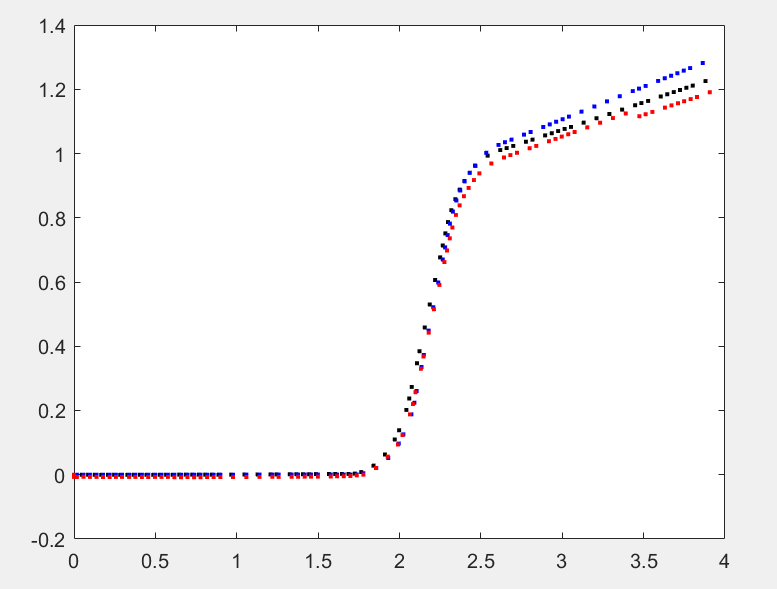
\includegraphics[width=0.45\textwidth]{images/T=30.png}}
                \hfill
                \subfloat[Results for running the simulation for $T=50$.]{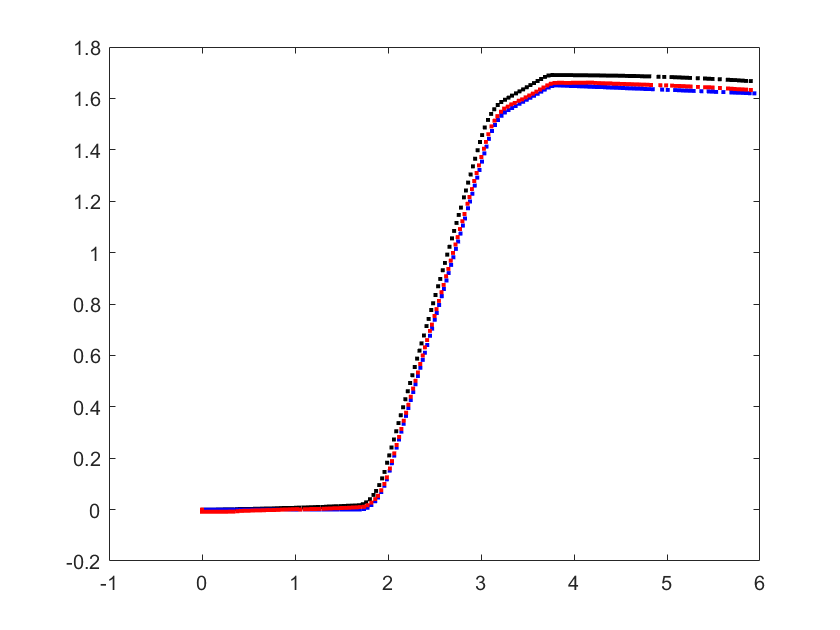
\includegraphics[width=0.45\textwidth]{images/T=50.png}}
                \caption{Comparison of simulation results for different time steps.}
            \end{figure}
        \end{solution}

        \part Discussion
        \begin{solution}
            As the time step increases, the EKF-based localization outperforms odometry due to its ability to correct errors. This results in more accurate and reliable positioning over time, as evidenced by the attached plots, whereas odometry leads to less precise localization due to error accumulated as the time increases. With the time increase, EKF and odometry both start getting further away from the actual path, however EKF-based localization is still closer to the actual path in comparison to the odometry.
        \end{solution}

        \part Measurement Uncertainty Covariance Matrix $R$
        \begin{solution}
            The measurement uncertainty covariance matrix $R$ is computed in the \texttt{extractLinesPolar.m} file.
            The covariance is being computed in the \texttt{fitLinePolar.m} file. After measuring $\rho$ and
            $\theta$ from the sensor, their covariance matrix and the relationship between $\rho$ and $\theta$,
            and $r$ and $\alpha$ is used to compute the Jacobian, which is then used to compute the covariance
            matrix $R$ using the error propagation formula:

            \(C_Y = F_X C_X F_X^T\)
        \end{solution}
    \end{parts}

    \question[20]
    Answer the following questions individually:
    \begin{parts}
        \part How many hours did each of you spend on this homework?
        \begin{solution}
            \subsection*{Ali Asghar Yousuf}
            36 hours

            \subsection*{Muhammad Azeem Haider}
            45 hours
        \end{solution}

        \part State each group member's specific contribution to this homework assignment.
        \begin{solution}
            \subsection*{Ali Asghar Yousuf}
            \begin{enumerate}
                \item Question 2
                \item Question 4
            \end{enumerate}

            \subsection*{Muhammad Azeem Haider}
            \begin{enumerate}
                \item Question 1
                \item Question 3
                \item Question 4
            \end{enumerate}
        \end{solution}

        \part Do you have any specific advice for students attempting this homework next year?
        \begin{solution}
            \subsection*{Ali Asghar Yousuf}
            Rushing through the homework is not a good idea, it is better to take your time
            and understand the concepts and then attempt the questions, otherwise you will
            end up wasting more time than you would have saved by rushing. In addition, it
            is better to start early and ask for help from the instructor and your peers if
            you are stuck on a question. Lastly, try enjoying the homework, it is a great
            way to learn and apply the concepts taught in class, and getting the results
            visualized really helps in understanding the concepts.

            \subsection*{Muhammad Azeem Haider}
            Start the homework early, you may look at the questions and tell yourself yeah
            these are simple questions, markov chains are not that difficult, and state
            estimation is not all that challenging but when you actually start doing the
            questions you realize you know too little and the questions really test your
            knowledge. Start early, no matter what your mind tells you. In addition, know
            your concepts, it is essential to know where you are struggling and fix it
            through this homework and take help from the instructor and your peers.

        \end{solution}

        \part Provide a self-reflection in the form of a note or a concept map.
        \begin{solution}
            \subsection*{Ali Asghar Yousuf}
            This homework was a great way to apply the concepts taught in class. It was
            challenging and required a lot of effort to complete. I learned a lot from this
            homework, especially about state estimation and how to apply it to real world
            problems. Applying the Kalman filter really helped me piece together the
            concepts taught in class and understand them better.

            \subsection*{Muhammad Azeem Haider}
            Attempting questions can often present a challenge, as they serve as practical
            applications following theoretical lectures. I initially approached Question 3,
            which appeared to be the most straightforward; however, it proved to be quite
            the contrary. Grasping the underlying principles of Markov chains and Bayesian
            estimation was a complex task. Furthermore, employing state estimation
            techniques to resolve the covariance matrix in question 1 added to the
            difficulty of the homework. The correctness of my approach to Question 1
            remains uncertain.

        \end{solution}
    \end{parts}
\end{questions}

\end{document}